\documentclass[11pt]{article}\usepackage[]{graphicx}\usepackage[]{color}
%% maxwidth is the original width if it is less than linewidth
%% otherwise use linewidth (to make sure the graphics do not exceed the margin)
\makeatletter
\def\maxwidth{ %
  \ifdim\Gin@nat@width>\linewidth
    \linewidth
  \else
    \Gin@nat@width
  \fi
}
\makeatother

\definecolor{fgcolor}{rgb}{0.345, 0.345, 0.345}
\newcommand{\hlnum}[1]{\textcolor[rgb]{0.686,0.059,0.569}{#1}}%
\newcommand{\hlstr}[1]{\textcolor[rgb]{0.192,0.494,0.8}{#1}}%
\newcommand{\hlcom}[1]{\textcolor[rgb]{0.678,0.584,0.686}{\textit{#1}}}%
\newcommand{\hlopt}[1]{\textcolor[rgb]{0,0,0}{#1}}%
\newcommand{\hlstd}[1]{\textcolor[rgb]{0.345,0.345,0.345}{#1}}%
\newcommand{\hlkwa}[1]{\textcolor[rgb]{0.161,0.373,0.58}{\textbf{#1}}}%
\newcommand{\hlkwb}[1]{\textcolor[rgb]{0.69,0.353,0.396}{#1}}%
\newcommand{\hlkwc}[1]{\textcolor[rgb]{0.333,0.667,0.333}{#1}}%
\newcommand{\hlkwd}[1]{\textcolor[rgb]{0.737,0.353,0.396}{\textbf{#1}}}%

\usepackage{framed}
\makeatletter
\newenvironment{kframe}{%
 \def\at@end@of@kframe{}%
 \ifinner\ifhmode%
  \def\at@end@of@kframe{\end{minipage}}%
  \begin{minipage}{\columnwidth}%
 \fi\fi%
 \def\FrameCommand##1{\hskip\@totalleftmargin \hskip-\fboxsep
 \colorbox{shadecolor}{##1}\hskip-\fboxsep
     % There is no \\@totalrightmargin, so:
     \hskip-\linewidth \hskip-\@totalleftmargin \hskip\columnwidth}%
 \MakeFramed {\advance\hsize-\width
   \@totalleftmargin\z@ \linewidth\hsize
   \@setminipage}}%
 {\par\unskip\endMakeFramed%
 \at@end@of@kframe}
\makeatother

\definecolor{shadecolor}{rgb}{.97, .97, .97}
\definecolor{messagecolor}{rgb}{0, 0, 0}
\definecolor{warningcolor}{rgb}{1, 0, 1}
\definecolor{errorcolor}{rgb}{1, 0, 0}
\newenvironment{knitrout}{}{} % an empty environment to be redefined in TeX

\usepackage{alltt}

\usepackage{epsilonj}
\RequirePackage{graphicx}
\usepackage{verbatim}
\RequirePackage[colorlinks,citecolor=blue,urlcolor=blue]{hyperref}

\addbibresource{../../template/epsilon.bib}
\IfFileExists{upquote.sty}{\usepackage{upquote}}{}
\begin{document}

\TITLE{Сгладить, нельзя не сгладить! Пара слов о методах сезонной корректировки}
\SHORTTITLE{Сгладить, нельзя не сгладить! Сезонная корректировка}

\AUTHOR{Иван Станкевич}{НИУ ВШЭ, Москва.}
\SHORTAUTHOR{Иван Станкевич}

\DoFirstPageTechnicalStuff

\begin{abstract}
В статье приводится обзор двух самых популярных на сегодняшний день процедур корректировки сезонности "--- методов семейства X-11 и TRAMO/SEATS. Описывается история развития методов, механизм их работы, указываются их основные достоинства и недостатки. Рассматривается реализация этих методов в компьютерных пакетах, в том числе \proglang{R}. 
\end{abstract}

\begin{keyword}
сезонность, R, X-11, X-12, TRAMO/SEATS
\end{keyword}


\section{В качестве введения}
\subsection{Зачем нужна сезонная корректировка}

Сезонность "--- очень распространенное в экономических (и не только) временных рядах явление, которому, увы, часто не уделяется достаточного внимания. Сезонность представляет собой регулярные колебания в данных, повторяющиеся из года в года примерно в одно и то же время. Что же является причиной сезонности? Прежде всего, это климатические и институциональные факторы, такие как выходные и праздничные дни (вспомним наши 10-дневные новогодние праздники в начале января, или 10 дней в начале мая, которые значимая часть населения страны проводит не на работе, а на даче, занимаясь сельскохозяйственными работами). Климат влияет на сельское хозяйство (тривиальным образом), потребление и производство электроэнергии (отопление зимой, в жарких и не только странах "--- кондиционирование летом), туризм, строительство; в меньшей степени "--- на добычу полезных ископаемых и отчасти на отдельные виды торговли и услуг. Некоторые авторы также выделяют как отдельную причину ожидания сезонности, которые в свою очередь провоцируют колебания, либо служат их усилению. 

Может возникнуть резонный вопрос, ответ на который не очевиден с первого взгляда, "--- зачем с ней бороться? На то есть целый ряд причин:

\begin{itemize}
\item Невозможность наблюдать и изучать тренды (особенно короткие, локальные тренды) в рядах с сильной сезонной компонентой. Проблема здесь в том, что сезонность, особенно сезонность с достаточно большой амплитудой, зачастую просто <<забивает>> тренд и рост или падение, к примеру, сельскохозяйственного производства на пару-тройку миллиардов рублей может просто пропасть на фоне сезонных колебаний размахом в сотни миллиардов. 
\item Высокая вероятность получения кажущихся зависимостей при оценке связи между рядами с сильной сезонностью (аналогично кажущимся регрессиям для нестационарных рядов). Если пики двух показателей приходятся на один квартал "--- отлично, корреляция будет большая и положительная, на разные "--- вполне возможно, что не менее большая и отрицательная. Но это, понятное дело, не говорит о наличии какой-то реальной зависимости между рядами. 
\item Проблемы с оценками коэффициентов из-за высокой дополнительной дисперсии. Чем выше дисперсия, тем, как мы знаем, ниже точность получаемых оценок, а чем ниже точность, тем хуже работают наши модели!
\item Трудности с обнаружением, анализом и предсказанием изломов в трендах и длинных циклах, особенно при использовании высокочастотных (месячных и чаще) данных. Проблема та же самая, что и с наблюдением коротких трендов, но в контексте не трендов, а их изломов. Кризис случился, а никто его и не заметил\ldots
\end{itemize}

Идейно есть два основных подхода к тому, что делать с сезонностью в данных (вариант <<не обращать внимание>> не рассматривается). Первый "--- это сезонная корректировка. При помощи тех или иных процедур из ряда явным образом выделяется сезонная компонента, которую после этого можно удалить и работать с данными, как обычно (к примеру, практически все статистические службы мира, в том числе и Росстат\footnote{Правда, Росстат публикует в сглаженном виде не так много рядов и обновляет их не каждый квартал, а раз в год}, публикуют основные макроэкономические ряды не только в исходном виде, но и в сглаженном). Второй подход "--- это моделирование сезонности, когда сезонные колебания учитываются при построении модели явным образом. К сожалению, сделать это получается не для всех моделей. 

Сезонная корректировка "--- самый простой способ работы с сезонностью в данных (особенно если корректировку проводит статистическая служба, а не исследователь), потому что не требует никаких дополнительных усилий со стороны исследователя (изучение структуры сезонности, изменение формы модели для учета сезонного фактора и т.д.). Оставляя в стороне самые простые варианты (классическую сезонную декомпозицию скользящими средними и взятие сезонных разностей "--- методы простые и хорошо работающие в некоторых приложениях, но не учитывающие многие нюансы, часто возникающие при работе с реальными данными разной природы), рассмотрим подробнее более современные методы. 

\subsection{Общие предпосылки}

Основное предположение об устройстве данных, которое делается процедурами сезонной корректировки и которое лежит, в конечном итоге, в основе всех методов удаления сезонности, заключается в следующем. Возьмём ряд данных $Y_t$. Тогда при использовании аддитивной модели сезонности верно равенство:

\[
Y_t = U_t + S_t + E_t
\]

Либо, при использовании мультипликативной модели сезонности:

\[ 
Y_t = U_t S_t E_t
\]

Где $U_t$ "--- трендовая компонента данных (долгосрочные тенденции), $S_t$ "--- сезонная компонента (циклы с периодом в год), $E_t$ "--- случайная составляющая (просто шум). Иногда в эту схему ещё добавляется четвертая компонента, отвечающая за более длинные циклы. 

В целом, такая схема предполагает, что данные можно разбить на три компоненты либо мультипликативно, либо аддитивно. Другие формы включения сезонности, как правило, не рассматриваются. В такой постановке задачи цель любой процедуры выделения сезонности "--- максимально точно оценить компоненту $S_t$, чтобы потом удалить её из данных. Надо понимать, что удаление сезонности, которое также иногда называют сглаживанием сезонности, "--- не совсем то же самое, что сглаживание данных. Сглаживание осуществляется с целью получения максимального гладкого ряда, где не будет не только периодических колебаний (хотя они как раз могут и остаться, в зависимости от того, как именно осуществляется сглаживание), но и шума (прежде всего шума). Сезонная корректировка же выделяет и удаляет только сезонную компоненту, случайную же она сохраняет, хотя современные процедуры, конечно, дают оценку и трендовой, и случайной составляющей по отдельности, что позволяет получать в том числе и гладкий тренд без шума. 

Теперь, поняв зачем нужна сезонная корректировка и в чем она, в конечном счете, заключается, можно переходить к описанию основных процедур, использующихся на практике. 
В этом небольшом обзоре сосредоточимся на двух наиболее часто использующихся: методах семейства X-11 и методе TRAMO/SEATS. 

\section{Методы семейства X-11} 
\subsection{Предыстория и X-11}

Методы семейства X-11 начали разрабатываться в US Bureau of Census ещё в далёкие 1950-ые годы, когда компьютеров было мало, а вычислительные мощности были серьёзно ограничены, что, в общем-то, наложило свой отпечаток на всё семейство процедур. Долгое время эти методы удаления сезонности из данных оставались основным инструментом и, во многом, остаются и по сей день. 

Общая идея процедуры достаточно проста - за несколько шагов, используя специальный набор фильтров и достаточно простой алгоритм, выделить оценки трендовой и сезонной компоненты ряда. Предлагались следующие шаги:

\begin{itemize}
\item На первом шаге осуществляется сглаживание для получения первоначальной оценки тренда. Здесь и далее "--- при помощи скользящей средней Хендерсона, про неё подробнее ниже.  Количество точек, по которому осуществляется сглаживание, зависит от частоты ряда (квартальный, месячный) и его характеристик. Полученная первоначальная оценка тренда удаляется из данных (в форме для мультипликативной сезонности): $\frac{Y_t}{\hat{U}_t} = \frac{U_t S_t E_t}{\hat{U}_t} \approx S_t E_t$
\item На втором шаге полученный на первом шаге ряд сглаживается для получения первоначальной оценки сезонности. Она удаляется из данных, получаем ряд:  $\frac{Y_t}{\hat{S}_t} = \frac{U_t S_t E_t}{\hat{S}_t} \approx U_t E_t$
\item На третьем шаге ряд, очищенный от первоначальной сезонности, сглаживается для получения второй оценки тренда, которая также удаляется из данных
\item Четвертый шаг "--- аналог второго, полученная оценка сезонности рассматривается как финальная
\item На пятом шаге из данных удаляется финальная оценка сезонности. Ряд сглаживается для получения финальной оценки тренда. 
\end{itemize}

В итоге получается разбиение ряда на трендовую компоненту, сезонную и нерегулярную. Шум "--- то, что осталось после удаления из данных сезонности и тренда. 

Есть ряд технических нюансов, которые следует помнить при работе с процедурами семейства X-11. 

Прежде всего, скользящие средние. В фильтрах X-11 используются скользящие средние Хендерсона\footnote{Henderson, R. (1916). Note on Graduation by Adjusted Average. Transactions of the American Society of Actuaries, 17, 43-48}, смысл которых в том, что если применить их к кубическому полиному (сгладить кубический полином при помощи скользящих средних Хендерсона), он не поменяется (сглаженный скользящими средними Хендерсона кубический полином должен быть идентичен тому же самому полиному, но не сглаженному). При этом веса у дальних наблюдений оказываются отрицательными (сумма всех весов, разумеется, равна единице). Как правило, считается, что кубического полинома (локального, конечно же, не в применении ко всему, возможно очень длинному, ряду) достаточно для описания экономических временных рядов, что оправдывает использование именно такого набора скользящих средних, и одновременно с этим скользящие средние Хендерсона достаточно эффективно удаляют высокочастотные шумы. 
Стоит заметить и ещё одну очень важную вещь - сглаживание на краях ряда осуществляется с использованием несимметричных (за отсутствием данных за пределами периода наблюдения) фильтров, что может порождать некоторые смещения (решение этой проблемы было предложено в версии X-11-ARIMA, о которой будет рассказано чуть ниже). 

Помимо собственно фильтра, в X-11 уже были встроены механизмы для борьбы с эффектом числа торговых дней (разное количество рабочих дней в разные месяцы и кварталы), с эффектами начала года и рядом других календарных эффектов, которые также оказывают заметное влияние на структуру сезонности. 

\subsection{X-11-ARIMA}

Метод X-11-ARIMA, предложенный Statistics Canada в 1980 году, предложил решение одной из самых серьёзных проблем исходного X-11 "--- проблемы краевых точек. Вместо использования несимметричных фильтров предлагалось достраивать ряд с концов при помощи оцененной по имеющимся данным ARIMA-модели и использовать обычные симметричные фильтры.\footnote{Можно, конечно, заметить, что все достроенные точки представляют собой не более чем линейную комбинацию старых, а значит и <<симметричный>> фильтр оказывается на самом деле несимметричным, но с весами, определяемыми по модели, а не заданными свыше} 

Подбор модели (заметим, что 1980 год был достаточно давно и вычислительные мощности по-прежнему были довольно ограниченными) осуществлялся достаточно любопытным образом. В процессе разработки метода, исследователи применяли большое количество моделей к большому количеству макроэкономических рядов, и выбрали среди этих моделей 5 наиболее универсальных, хорошо работающих в большинстве случаев (хотя бы одна из них хорошо работала в подавляющем большинстве случаев). Вот эти модели:

\begin{center}
\begin{tabular}{ccccc}
ARIMA(0,1,1) x SARIMA(0,1,1) \\
ARIMA(0,1,2) x SARIMA(0,1,1) \\
ARIMA(2,1,0) x SARIMA(0,1,1) \\
ARIMA(0,2,2) x SARIMA(0,1,1) \\
ARIMA(2,1,2) x SARIMA(0,1,1) \\
\end{tabular}
\end{center}

Где в записи ARIMA(p,d,q) x SARIMA(P,D,Q): $p$ "--- количество обычных AR лагов, $P$ "--- количество сезонных AR лагов (первый сезонный лаг "--- 4-ый лаг для квартальных данных, 12-ый для месячных и так далее); аналогично $d$ и $D$ "--- разности обычные и сезонные; $q$ и $Q$ "--- MA лаги. К примеру, модели ARIMA(0,1,1) x SARIMA(0,1,1) для месячных данных будут записываться следующим образом:

\[
(1 - \Delta)(1 - \Delta^{12})Y_t = (1 - \beta_1 \Delta)(1 - \beta_2 \Delta^{12}) \varepsilon_t
\]

Метод X-11-ARIMA использует следующий алгоритм получения скорректированного ряда: 

\begin{itemize}
\item На первом шаге очищает данные от календарных эффектов "--- торговые дни, начало года, <<гуляющие>> праздники типа Пасхи и т.д.
\item На втором "--- строит по данным ARIMA-модели. При этом процедура оценивает все пять моделей из списка, оставляет те из них, которые удовлетворяют минимальным критериям по точности, значимости статистик Бокса-Льюнга (они должны быть незначимыми для лагов, соответствующих 2 годам "--- 8 кварталов или 24 месяца) и не передифференцируют (не берут слишком много разностей) ряды. Из моделей, прошедших отбор, выбирается лучшая на основе критерия MAPE (Mean Absolute Percent Error): $MAPE = 100\% \frac{1}{n} \sum_{t = 1}^n \frac{|y_t - \hat{y}_t|}{|y_t|}$. При этом прогнозы каждый раз строятся на 1 шаг вперед, потом ряд дополняется одной точкой из реальных данных и опять строится прогноз на 1 шаг вперед. 
\item Ряд достраивается с краев до длины, достаточной для использования обычного симметричного фильтра X-11
\item Наконец, фильтр X-11 применяется к достроенному ряду, получаются оценки трендовой, сезонной и нерегулярной компонент. 
\end{itemize}

\subsection{X-12-ARIMA и дальнейшее развитие}

Следующей важной вехой на пути развития методов семейства X-11 был метод X-12-ARIMA (который используется и по сей день), предложенный уже в 1990 году. Главным нововведением было использование моделей regARIMA:

\[
\ln\left(\frac{Y_t}{D_t}\right) = \beta' X_t + Z_t
\]

Где $Y_t$ "--- ряд данных, $D_t$ "--- преобразования в данных (какие-то априорные сведения о структуре сезонности, которыми мы располагаем), $X_t$ - матрица регрессоров (количество торговых дней, дамми на праздники, в том числе плавающие, и другие календарные эффекты "--- использование этих переменных внутри модели и есть главное нововведение моделей regARIMA), $Z_t$ "--- ARIMA процесс. 

Модели regARIMA - логичное продолжение идей метода X-11-ARIMA, позволяющее в рамках одной конструкции учесть и календарные эффекты, и оценить по данным ARIMA (SARIMA) модель. При помощи этой же модели осуществляется поиск выбросов, достраиваются пропуски в данных (возможность работать с данными с пропусками также является важным достижением метода), явно оцениваются календарные эффекты, что также может представлять интерес. 
При этом выбор модели может осуществляться как аналогично модели X-11-ARIMA, из списка (правда, здесь он заметно больше), так и автоматически "--- начиная с самой простой модели с постепенным добавлением лагов и разностей, пока это улучшает качество модели. Такой подход позволяет не ограничивать выбор моделей каким-то списком, что потенциально делает метод применимым ещё в большем количестве ситуаций, в том числе достаточно экзотических. 

Помимо этого, в пакет встроено большое количество дополнительных функций для диагностики данных (спектральный анализ, средства для анализа стабильности сезонности и качества работы сезонной корректировки), что также можно отнести к достоинствам пакета, потому что это экономит время и силы исследователя. 

Последняя на сегодня версия пакета "--- X-13-ARIMA-SEATS\footnote{Сама программа, её документация, новости и много чего ещё доступно на сайте US Bureau of Census, \url{https://www.census.gov/srd/www/x13as/}}. Если не получается на него зайти (из России иногда возникают проблемы с доступом к сайту census.gov) "--- можно попробовать воспользоваться прокси\footnote{Например, \url{https://hide.me/en/proxy} или \url{https://www.hidemyass.com/proxy}} или Tor "--- в целом сохраняет функционал X-12-ARIMA, но добавляет к нему возможность пользоваться методом SEATS (о нём чуть ниже) из того же пакета. 

\section{TRAMO/SEATS} 

Процедура TRAMO/SEATS (строго говоря, не столько процедура, сколько набор из двух программ "--- собственно TRAMO и SEATS, "--- которые предлагается использовать в комплексе) была предложена центральным банком Испании (Bank of Spain) в 1996 году. Она основана на идеях, заметно отличающихся от использующихся в методах семейства X-11. Прежде всего "--- это подбор фильтра на основе данных, а не использование готового универсального решения, как в X-11. Две части метода решают две разные задачи. 

TRAMO (Time Series Regression with ARIMA Noise, Missing Observations and Outliers) по сути своей аналогичен моделям regARIMA. Здесь так же строится регрессия исходных данных на календарные переменные с остатками в форме ARIMA, так же определяются и корректируются выбросы в данных. 

SEATS (Signal Extraction in ARIMA Times Series) значительно интереснее. Она рассматривает остатки $Z_t$ из regARIMA (TRAMO) как сумму трёх компонент (вспомним аддитивную модель сезонности):

\[
Z_t = U_t + S_t + E_t
\]

Как и раньше, $U_t$ "--- тренд, $S_t$ "--- сезонность, $E_t$ "--- нерегулярная компонента.

И вводит ряд дополнительных предпосылок (ортогональность $U_t$ и $S_t$, белошумность $E_t$). Тогда, зная модель для $Z_t$ (из оценок TRAMO), процедура получает в явном виде модели для $U_t$ и $S_t$. Это делается не единственным образом, но можно отобрать <<лучшую>> по какому-то критерию "--- здесь минимизируется шум в $S_t$. Полученные таким образом модели можно использовать для фильтрации рядов. 

Более подробно описывать устройство TRAMO/SEATS в рамках обзорной статьи смысла нет, но если возникнет необходимость более глубоко погрузиться в нюансы его работы "--- стоит ознакомиться с документацией на сайте Банка Испании\footnote{\url{http://www.bde.es/bde/en/secciones/servicios/Profesionales/Programas_estadi/Notas_introduct_3638497004e2e21.html}, правда, стоит заметить, что качество этой документации оставляет желать лучшего}, и со статьями, посвященными этому вопросу: хорошая подборка есть там же, на сайте Банка Испании\footnote{\url{http://www.bde.es/bde/en/secciones/servicios/Profesionales/Programas_estadi/Trabajos_sobre__0ac07f3710fd821.html}}. 


\begin{figure}[hbtp]
\centering
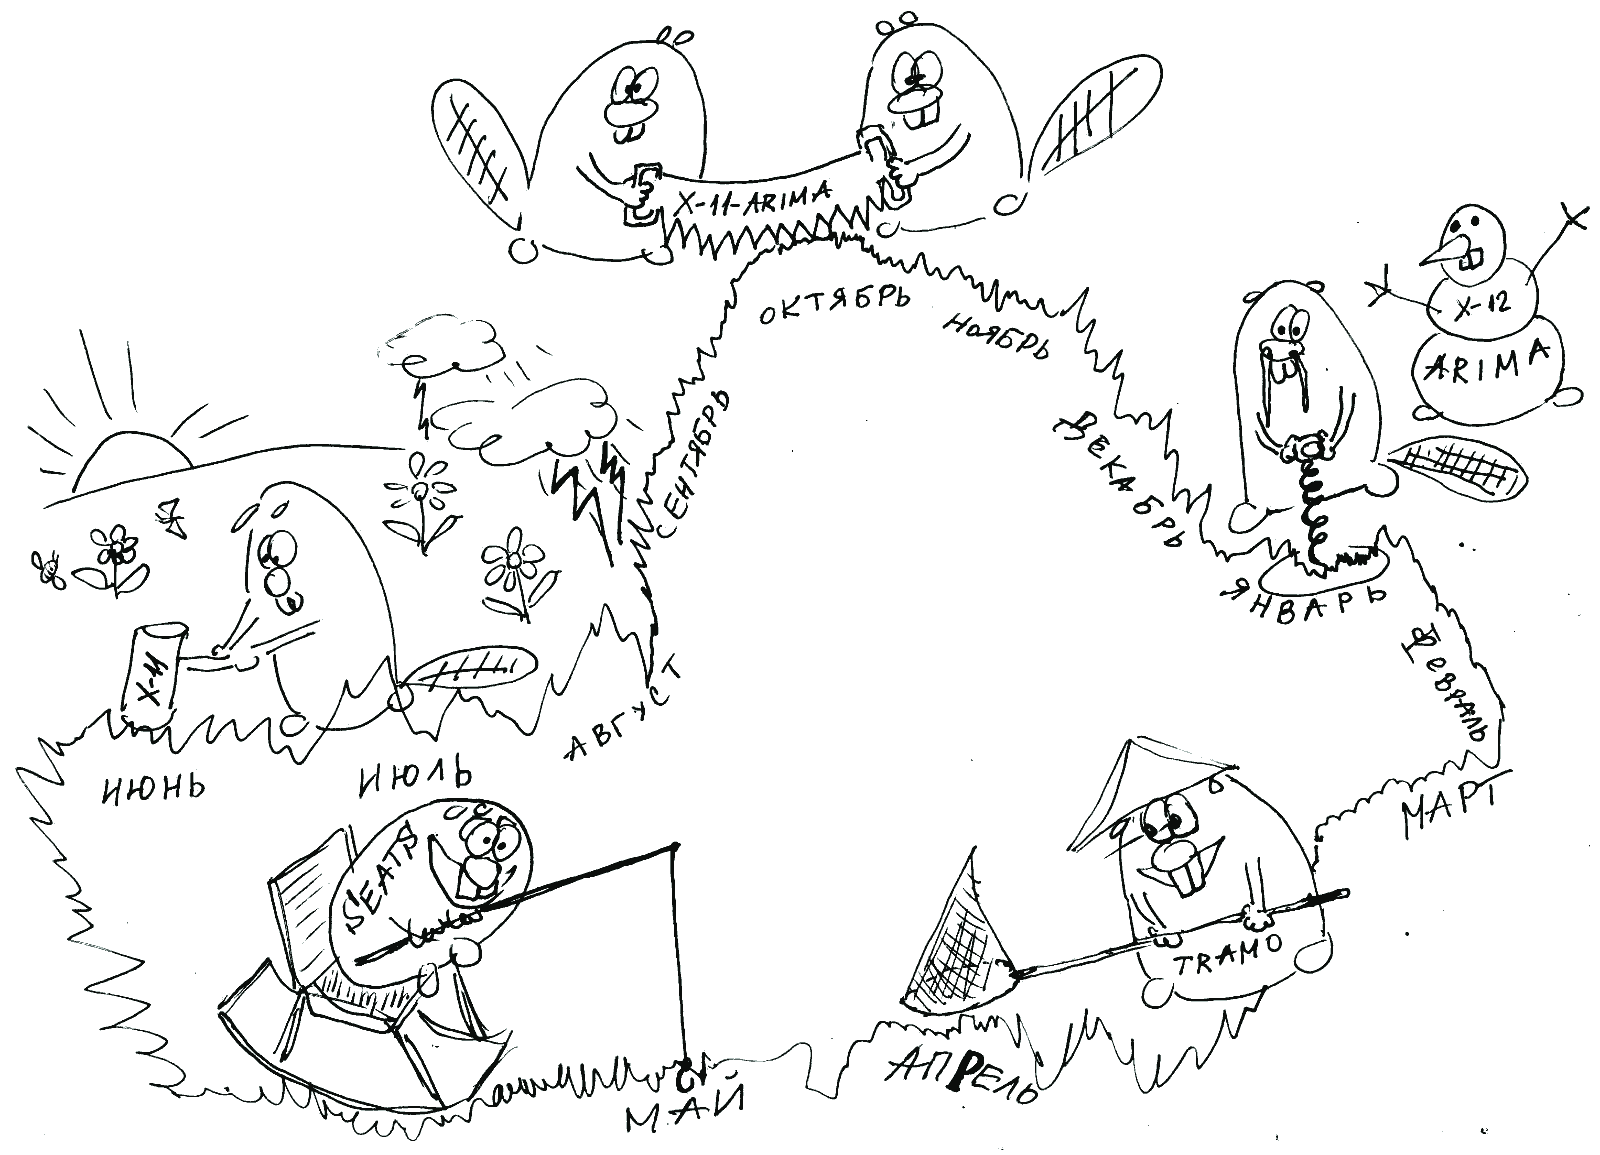
\includegraphics[width=10cm]{bobr_final.png}
\caption{Бобры выполняют сезонную корректировку}
\end{figure}

\section{Общие слова}
\subsection{О преимуществах и недостатках методов}

Методы семейства X-11 и TRAMO/SEATS представляют два основных направления в области сезонной корректировки "--- использование наборов готовых фильров и определение оптимального фильтра по данным. Каждый из подходов имеет свои достоинства и недостатки. 

Методы X-11 считаются более гибкими, потому что используют непараметрический подход, не специфицируя форму сезонности ни в какой форме, тогда как SEATS предполагает, что сезонность задаётся линейной ARIMA моделью. Поэтому метод TRAMO/SEATS, как раз благодаря сравнительно жёсткой параметризации зависимостей, может оказаться более точным в некоторых ситуациях. Последние версии американской процедуры также предлагают большое количество дополнительных функций для диагностики сезонности в данных, чем не может похвастаться процедура европейская. При этом считается, что на практике TRAMO/SEATS иногда даёт более гладкие результаты, и более устойчивые к добавлению новых точек, а X-11 лучше работает на сравнительно коротких (до 5-6 лет) временных рядах. 

При этом для многих сравнительно простых случаев разница между X-12 и TRAMO/SEATS остается практически незаметной. К примеру, на графике 1 приведен квартальный ВВП России в текущих ценах в исходном виде и скорректированный X-12-ARIMA и TRAMO/SEATS, а на рисунке 2 "--- расхождение в рядах, скорректированных этими двумя методами. Как видно, расхождения очень невелики, хотя и носят очевидно неслучайный характер, обусловленный разными свойствами методов. Следовательно, и больших различий в выводах, полученных по этим данным, скорее всего, не будет. 

\begin{figure}
\centering
\subfigure[{Динамика ВВП в исходном виде и скорректированного X"~12 и TRA\-MO\slash SEATS}]{
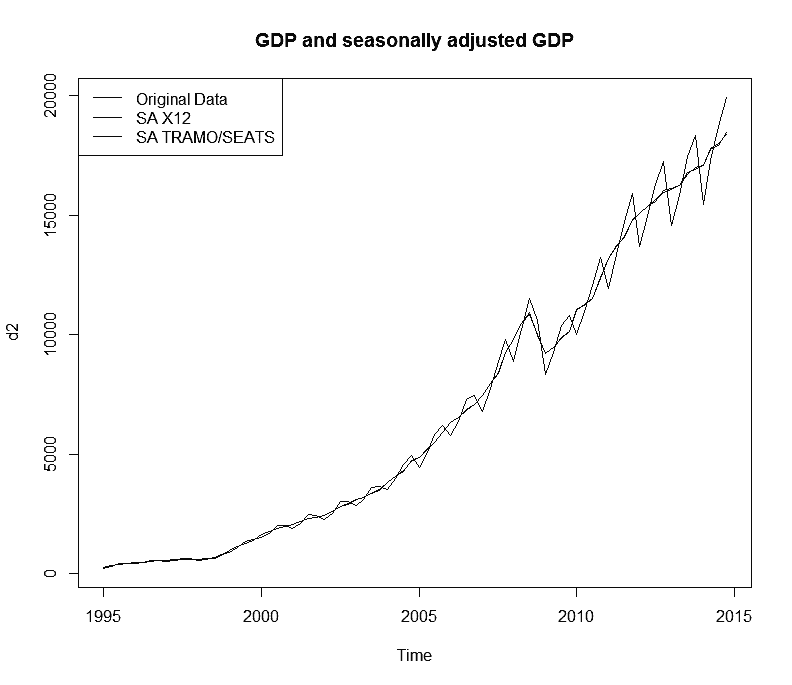
\includegraphics[width=5cm]{eps_seas1.png}\label{fig:test1}
}
\quad
\subfigure[{Расхождение в рядах, скорректированных X-12 и TRA\-MO\slash SEATS}]{
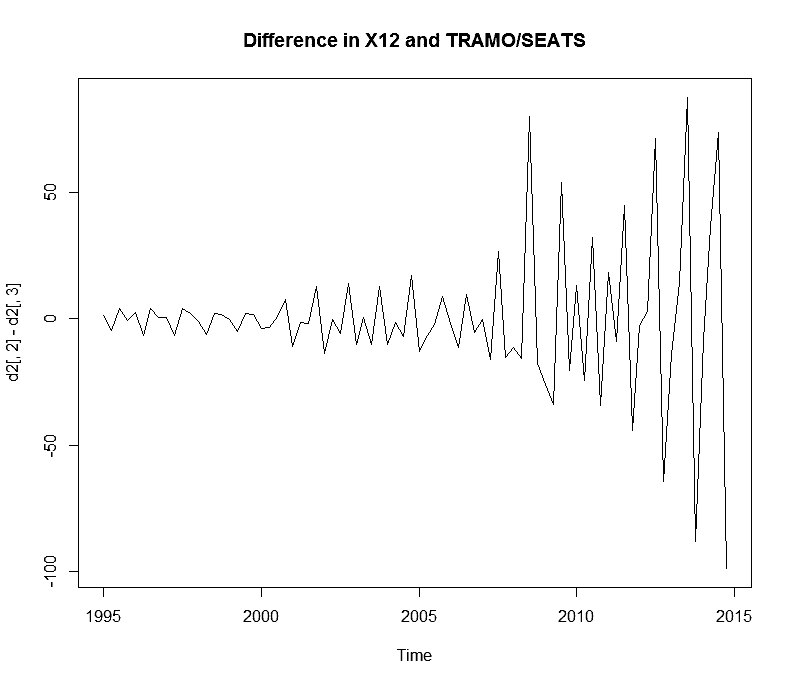
\includegraphics[width=5cm]{eps_seas2.png}\label{fig:test2}
}
\end{figure}

В целом же, выбор лучшего метода для сезонной корректировки остаётся процессом во многом творческим и требующим как понимания методов, так и вдумчивой работы с данными. 

\subsection{Реализация в компьютерных пакетах}

Из коммерческих пакетов в~\proglang{EViews 8} доступны и X-13, и TRAMO/SEATS; в \proglang{STATA}, насколько известно автору, доступность ограничивается версией X-12-ARIMA, TRAMO/SEATS также доступен. 

В~\proglang{R} доступны все методы и в разных версиях. Есть отдельный пакет \pkg{x12} для X-12-ARIMA,
%\footnote{\href{http://cran.r-project.org/web/packages/x12/x12.pdf}{Так и называется, \pkg{x12}}}
достаточно удобный, правда, не так давно разработчики достаточно сильно поменяли синтаксис, из-за чего автору пришлось переписывать много кода, и, если они сделали это один раз, ничего не мешает им сделать это ещё раз\footnote{В таких ситуациях можно ставить пакеты \proglang{R} на определённую дату с помощью пакетов \pkg{packrat} или \pkg{checkpoint}.}. 

Для нового метода X-13 также есть отдельный пакет \pkg{seasonal},
%\footnote{\href{http://cran.r-project.org/web/packages/seasonal/seasonal.pdf}{Называется \pkg{seasonal}}}
тоже новый. Он позиционируется как простой и удобный в использовании. 

Важно отметить, что все пакеты для методов семейства X-11 требуют установки исходных двоичных файлов (binaries), которые можно бесплатно и без регистрации скачать на сайте Bureau of Census, \href{http://www.census.gov/srd/www/x12a/}{www.census.gov/srd/www/x12a/}. После установки, в \proglang{R} надо будет просто указать путь к этим файлам. 

Пакет для работы с TRAMO/SEATS в \proglang{R}  (и не только) есть на сайте Банка Испании, \url{http://www.bde.es/bde/en/secciones/servicios/Profesionales/Programas_estadi/Interfaces.html}. Представлено как описание пакета, так и простейшие примеры работы с ним. 

\subsection{Почему надо быть осторожными при использовании сезонной корректировки}

Несмотря на все достоинства методов сезонной корректировки с точки зрения простоты использования и минимизации дополнительных усилий исследователя, стоит заметить, что у них есть и ряд серьёзных недостатоков, исследованию которых посвящен большой пласт литературы. Рассмотрим некоторые из них. 

Самая, пожалуй, неожиданная черта процедур сезонной корректировки "--- это их способность создавать фиктивную сезонность.\footnote{Бессонов В. А., Петроневич А. В. Сезонная корректировка как источник ложных сигналов1 //Экономический журнал ВШЭ. – 2013. – Т. 17. – №. 4. – С. 554-584} Смысл в том, что если пропустить через алгоритм сезонной корректировки ряд без сезонности, но с выбросом, на <<очищенных>> от сезонности рядах в окрестности этого выброса методы (это свойственно как семейству X-11, так и TRAMO/SEATS) покажут ложные волны, очень похожие на неучтенную сезонность. В контексте анализа реальных данных эта проблема становится ещё серьезнее "--- на скорректированных рядах, содержащих, к примеру, кризисный период, в окрестности кризиса (самое главное "--- перед кризисом) появятся какие-то волны, которые можно трактовать в том числе и как предвестники кризиса. После чего следует вывод, что кризис приближался, это было заметно, но никто не обратил на него внимания, тогда как на самом деле эти <<предвестники кризиса>> "--- не более чем артефакты процедур сезонной корректировки. 

Ещё одна достаточно серьёзная проблема процедур удаления сезонности "--- это создаваемые ими смещения в тестах на единичные корни. Было аналитически доказано,\footnote{Ghysels E., Perron P. The effect of seasonal adjustment filters on tests for a unit root //Journal of Econometrics. – 1993. – Т. 55. – №. 1. – С. 57-98.} что в случае отсутствия единичного корня в данных сезонная корректировка создает смещение в тестах в сторону наличия единичного корня. То есть, стационарный ряд после сезонной корректировки можно принять за нестационарный! И чем дальше ряд от нестационарного - тем больше смещение. Та же самая проблема получается и при тестировании на коинтеграцию при помощи теста Энгла-Грейнджера. При этом для нестационарных рядов никаких дополнительных эффектов не возникает. 

Большое количество проблем также возникает в связи с шоками, выбросами и сдвигами в данных. К примеру, было показано,\footnote{Matas-Mir A., Osborn D. R., Lombardi M. J. The effect of seasonal adjustment on the properties of business cycle regimes //Journal of Applied Econometrics. – 2008. – Т. 23. – №. 2. – С. 257-278.} что сезонная корректировка при наличии в данных шока длиной в несколько точек (чего-то наподобие кризиса) уменьшает величину шока, но увеличивает его продолжительность и сдвигает точку окончания спада (а это уже действительно серьёзная с точки зрения, к примеру, проведения государственной политики, проблема). X-12-ARIMA часто оказывается неустойчивым к выбросам и структурным сдвигам,\footnote{Bruce A. G., Jurke S. R. Non-Gaussian seasonal adjustment: X-12-ARIMA versus robust structural models //Journal of Forecasting. – 1996. – Т. 15. – №. 4. – С. 305-328} на коротких рядах может создавать смещения в начале ряда, которые растут с ростом волатильности сезонной компоненты.\footnote{Mir A. M., Rondonotti V. The performance of X-12 in the seasonal adjustment of short time series //Seasonal Adjustment. – 2003. – С. 149.}

И этим список проблем, порождаемых сезонной корректировкой, не исчерпывается. Разумеется, это не значит, что сезонную корректировку нельзя использовать ни в коем случае и ни под каким предлогом, но равно не стоит и применять её бездумно ко всем рядам и безоглядно доверять получившимся результатам. Во многих ситуациях может оказаться разумнее вместо сезонной корректировки просто построить модель, в явном виде учитывающую сезонность, либо же внимательнее изучить и сравнить свойства разных процедур сезонной корректировки в контексте тех проблем и особенностей, которые свойственны изучаемым рядам. 

\section{Небольшая инструкция по установке}


\subsection{Установка на windows}

\begin{enumerate}
\item Скачайте готовый архив \verb|x13ashtmlall.zip| с \url{http://www.census.gov/srd/www/x13as/x13down_pc.html}. Если буржуйский сайт блокируется доблестными силами добра (например, у меня блокируется втихаря, как будто такого сайта нет, без предупреждения <<Ресурс заблокирован\ldots>>), то можно воспользоваться сервисами веб-прокси. Например, \url{https://hide.me/en/proxy}, \url{https://www.hidemyass.com/proxy} и т.д.
\item Распакуйте архив и запомните адрес папки с файлом \verb|x13ashtml.exe|.
\item Установите в \proglang{R}  пакет \pkg{seasonal}.
\end{enumerate}

\subsection{Установка на macos/linux}

Подробная инструкция есть на странице \url{https://github.com/christophsax/seasonal/wiki/}. Борьба с блокировкой буржуйского сайта также может потребоваться :)


\subsection{Простой пример}
В начале скрипта \proglang{R}  мы пишем
\begin{knitrout}
\definecolor{shadecolor}{rgb}{0.969, 0.969, 0.969}\color{fgcolor}\begin{kframe}
\begin{alltt}
\hlkwd{Sys.setenv}\hlstd{(}\hlkwc{X13_PATH} \hlstd{=}\hlstr{"путь к папке с файлами"}\hlstd{)}
\hlkwd{library}\hlstd{(}\hlstr{"seasonal"}\hlstd{)}
\end{alltt}
\end{kframe}
\end{knitrout}

Если есть желание проверить, что всё ок, то это можно сделать командой \code|checkX13()|. И простой-простой пример автоматической борьбы с сезонностью в ряду~\code|y|:
\begin{knitrout}
\definecolor{shadecolor}{rgb}{0.969, 0.969, 0.969}\color{fgcolor}\begin{kframe}
\begin{alltt}
\hlstd{y_sa_model} \hlkwb{<-} \hlkwd{seas}\hlstd{(y)}
\hlstd{y_sa} \hlkwb{<-} \hlkwd{final}\hlstd{(y_sa_model)}
\end{alltt}
\end{kframe}
\end{knitrout}

Список \code|y_sa_model| будет содержать модель, которая использовалась для корректировки сезонности, а ряд \code|y_sa| будет очищенным от сезонности.

На сайте \url{https://github.com/christophsax/seasonal/wiki/} есть куча примеров! Прочитайте также замечательную виньетку к пакету \pkg{seasonal}, \url{http://cran.r-project.org/web/packages/seasonal/vignettes/seas.pdf}, там есть и инструкция по установке, и графический интерфейс для подбора модели корректировки сезонности!


\section{Выводы}

Сезонная корректировка "--- один из основных инструментов работы с сезонностью в данных. Она позволяет быстро и удобно устранить сезонность и продолжать работать с данными. Два основных метода устранения сезонности "--- методы семейства X-11 и TRAMO/SEATS "--- применяют несколько отличные подходы (которые описаны выше и которые полезно хотя бы в общих чертах понимать, чтобы не работать с процедурами как с <<чёрными ящиками>>, как это, увы, чаще всего происходит). Оба метода представлены во всех основных статистических пакетах, как коммерческих, так и открытых. Оба же метода иногда приводят к появлению дополнительных проблем в данных, о которых следует помнить и которые следует учитывать при использовании сезонно скорректированных данных.


\end{document} 


